\pdfoutput=1
% In particular, the hyperref package requires pdfLaTeX in order to break URLs across lines.

\documentclass[11pt]{article}

% Change "review" to "final" to generate the final (sometimes called camera-ready) version.
% Change to "preprint" to generate a non-anonymous version with page numbers.
\usepackage[preprint]{acl}

% Standard package includes
\usepackage{times}
\usepackage{latexsym}

% For proper rendering and hyphenation of words containing Latin characters (including in bib files)
\usepackage[T1]{fontenc}
% For Vietnamese characters
% \usepackage[T5]{fontenc}
% See https://www.latex-project.org/help/documentation/encguide.pdf for other character sets

% This assumes your files are encoded as UTF8
\usepackage[utf8]{inputenc}

% This is not strictly necessary, and may be commented out,
% but it will improve the layout of the manuscript,
% and will typically save some space.
\usepackage{microtype}

% This is also not strictly necessary, and may be commented out.
% However, it will improve the aesthetics of text in
% the typewriter font.
\usepackage{inconsolata}

%Including images in your LaTeX document requires adding
%additional package(s)
\usepackage{graphicx}
\usepackage{hyperref}

% If the title and author information does not fit in the area allocated, uncomment the following
%
%\setlength\titlebox{<dim>}
%
% and set <dim> to something 5cm or larger.

\title{Etude comparative de vecteurs pour l'identification du parti politique d'interventions parlementaires}

% Author information can be set in various styles:
% For several authors from the same institution:
\author{Pauline Degez \and Florian Philippe \and Valentine Fleith \\
         43004729@parisnanterre.fr \\ 40007675@parisnanterre.fr \\ 43017467@parisnanterre.fr}
% if the names do not fit well on one line use
%         Author 1 \\ {\bf Author 2} \\ ... \\ {\bf Author n} \\
% For authors from different institutions:
% \author{Author 1 \\ Address line \\  ... \\ Address line
%         \And  ... \And
%         Author n \\ Address line \\ ... \\ Address line}
% To start a separate ``row'' of authors use \AND, as in
% \author{Author 1 \\ Address line \\  ... \\ Address line
%         \AND
%         Author 2 \\ Address line \\ ... \\ Address line \And
%         Author 3 \\ Address line \\ ... \\ Address line}

%\author{First Author \\
  %Affiliation / Address line 1 \\
  %Affiliation / Address line 2 \\
  %Affiliation / Address line 3 \\
  %\texttt{email@domain} \\\And
  %Second Author \\
  %Affiliation / Address line 1 \\
  %Affiliation / Address line 2 \\
  %Affiliation / Address line 3 \\
  %\texttt{email@domain} \\}

%\author{
%  \textbf{First Author\textsuperscript{1}},
%  \textbf{Second Author\textsuperscript{1,2}},
%  \textbf{Third T. Author\textsuperscript{1}},
%  \textbf{Fourth Author\textsuperscript{1}},
%\\
%  \textbf{Fifth Author\textsuperscript{1,2}},
%  \textbf{Sixth Author\textsuperscript{1}},
%  \textbf{Seventh Author\textsuperscript{1}},
%  \textbf{Eighth Author \textsuperscript{1,2,3,4}},
%\\
%  \textbf{Ninth Author\textsuperscript{1}},
%  \textbf{Tenth Author\textsuperscript{1}},
%  \textbf{Eleventh E. Author\textsuperscript{1,2,3,4,5}},
%  \textbf{Twelfth Author\textsuperscript{1}},
%\\
%  \textbf{Thirteenth Author\textsuperscript{3}},
%  \textbf{Fourteenth F. Author\textsuperscript{2,4}},
%  \textbf{Fifteenth Author\textsuperscript{1}},
%  \textbf{Sixteenth Author\textsuperscript{1}},
%\\
%  \textbf{Seventeenth S. Author\textsuperscript{4,5}},
%  \textbf{Eighteenth Author\textsuperscript{3,4}},
%  \textbf{Nineteenth N. Author\textsuperscript{2,5}},
%  \textbf{Twentieth Author\textsuperscript{1}}
%\\
%\\
%  \textsuperscript{1}Affiliation 1,
%  \textsuperscript{2}Affiliation 2,
%  \textsuperscript{3}Affiliation 3,
%  \textsuperscript{4}Affiliation 4,
%  \textsuperscript{5}Affiliation 5
%\\
%  \small{
%    \textbf{Correspondence:} \href{mailto:email@domain}{email@domain}
%  }
%}

\begin{document}
\maketitle
\begin{abstract}
Dans cette étude, nous avons exploré trois techniques de vectorisation différentes (TF-IDF, Doc2Vec et embeddings BERT) ainsi que quatre algorithmes d'apprentissage automatique (Random Forest, SVM, Régression Logistique et Perceptron) pour réaliser la tâche 3 de la cinquième édition du défi DEFT'09 (Défi Fouille de Texte 2009). Notre objectif était de comparer les performances des différents types de vectorisation dans une tâche de classification de texte, et de nous confronter aux résultats de 2009 (0.33 f-mesure). En définitive, le modèle SVM avec des vecteurs TF-IDF s'est révélé le plus performant (0.47). Les résultats obtenus avec les embeddings BERT, en revanche, se sont avérés plutôt décevants, bien qu'ils pourraient être améliorés par un fine-tuning pour mieux prendre en compte la spécificité du corpus.
\end{abstract}

% \section{Introduction}
\section{Introduction}

\par La cinquième édition du défi Fouille de Textes (DEFT) porte sur la fouille d'opinions sur des corpus multilingues. Trois tâches ont été proposées,
dans trois langues : le français, l'anglais et l'italien. Cet article se concentre sur la 3ème tâche, dont l'objet est l'identification automatique
du parti politique d'appartenance de chacun des intervenants dans un corpus de débats parlementaires européens. Il s'agit d'une tâche de classification à 5 classes:
\texttt{Verts-ALE}, \texttt{GUE-NGL}, \texttt{PSE}, \texttt{ELDR} et \texttt{PPE-DE}.

\par Le but de nos expériences sera ainsi de trouver un/des classifieur(s) permettant de réaliser cette tâche. Pour ce faire, nous utiliserons les algorithmes
de Machine Learning implementés dans la bibliothèque Python \texttt{scikit-learn}.

\subsection{Travaux présentés en 2009}




\begin{table}[h!]
\centering
\setlength{\tabcolsep}{5pt} % Réduit l'espace entre les colonnes
\renewcommand{\arraystretch}{1.2} % Ajuste la hauteur des lignes
\resizebox{\columnwidth}{!}{ % Ajuste la largeur à une demi-colonne
\begin{tabular}{@{}c| c| c| c| c| c@{}}
\textbf{Parti} & \textbf{ELDR} & \textbf{GUE-NGL} & \textbf{PPE-DE} & \textbf{PSE} & \textbf{Verts/ALE} \\
\hline
F-mesure & 0.21 & 0.37 & 0.47 & 0.37 & 0.25 \\ 
\end{tabular}
}
\caption{Moyennes des F-mesures par parti politique.}
\label{tab:moyennes_fmesures}
\end{table}


\par En 2009, un seul participant a soumis un travail pour la tâche 3 ; la Présentation de l'édition 2009 \hyperlink{ref1}{[1]}\footnote{Actes du cinquième défi fouille de texte, DEFT2009, Paris, France, 22 juin 2009} évoque, pour expliquer cela, les faibles résultats des logiciels sur cette tâche, bien que conformes à ceux que des humains obtiendraient manuellement. L'équipe de l'Université de Montréal (D. Forest and al.) a obtenu en moyenne les f-mesures présentées dans la \hyperref[tab:moyennes_fmesures]{Table 1}. En moyenne, cela donne donc une f-mesure 0.331.

\subsection{Notre approche et travaux antérieurs}

Pour ce travail, notre approche a été comparative sur plusieurs niveaux. Tout d'abord, nous comparons différents classifieurs : \texttt{Random Forest}, \texttt{Régression logistique}, \texttt{Perceptron} et \texttt{Support Vector Machine}. De plus, nous testons aussi différentes vectorisations du corpus sur l'ensemble de ces modèles: \texttt{TF-IDF}, \texttt{Doc2Vec}, et des \texttt{Bert embeddings}.


\par Plusieurs travaux de recherches explorent les comparaisons entre performances des modèles selon les techniques de vectorisation utilisées. Nous pouvons par exemples évoquer ceux de P. Joseph et S. Y. Yerima~\hyperlink{ref1}{[1]} \footnote{P. Joseph and S. Y. Yerima, "A comparative study of word embedding techniques for SMS spam detection," 2022 14th International Conference on Computational Intelligence and Communication Networks (CICN), Al-Khobar, Saudi Arabia, 2022, pp. 149-155,} en 2022, qui compare les performances des N-grams, TF-IDF, Sac de mots, Word2Vec, Doc2Vec, etc. Leur objectif est de comparer l'impact de la vectorisation sur la précision des modèles. Dans leur article, les modèles \texttt{Doc2Vec} et \texttt{TF-IDF} démontrent de bons résultats, nous allons ainsi les tester dans notre expérience. Nous décidons d'ajouter à ces deux dernier les embeddings de \texttt{BERT} afin d'avoir trois techniques variées : une méthode statistique, une méthode fondée sur un ANN classique et une sur un Transformer.




% \section{Engines}
\section{Méthode}

\subsection{Dataset}

Nous utilisons le dataset fournit pour la tâche 3 de l’édition 2009 de DEFT.
Il s'agit d'un corpus multilingue de débats parlementaires européens. Chaque intervention
parlementaire est classée en fonction du parti \footnote {ELDR, PPE-DE, PSE, GUE-NGL et Verts-ALE}
du locuteur et présente dans le corpus dans 3 langues : anglais, français et italien.\\
Au moment de faire des statistiques descriptives, nous nous sommes rendus comptes 
que le corpus présentait des doublons, et ce majoritairement dans la partition test.
\begin{figure}[ht]
    \centering
    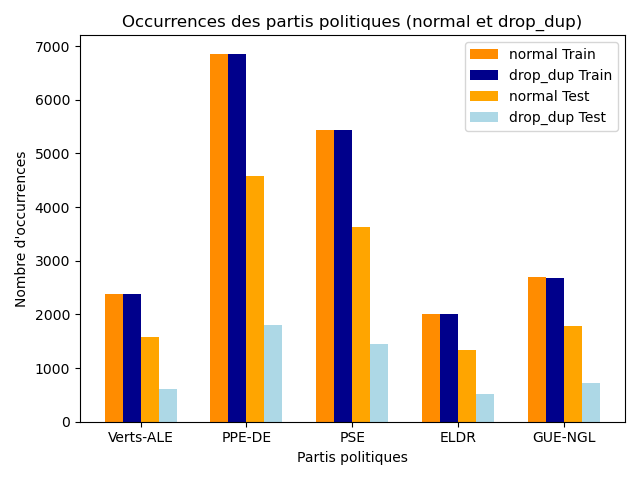
\includegraphics[width=\columnwidth]{../stats/occurences_orig_vs_drop_dup_par_cat.png}
    \caption{Nombre d'interventions par parti par partition test/train, dans le corpus original et dans la version sans doublons}
    \label{fig:barplot_dataset}
\end{figure}

Après suppression des doublons, la partition prévu (40/60) est changée : elle est 
maintenant de 20/80\footnote{ 0.79 pour le train et 0.21 pour le test}.
Nous avons envisagé de refaire le partitionnement pour réimplémenter le partitionnement 
prévu, mais avons renoncé pour deux raisons : 
refaire le partitionnement nous éloigne, encore, du corpus initialement prévu, et les 
résultats de quelques modèles sur un corpus repartitionné étaient proches des résultats 
sur cette partition 80/20.
Par ailleurs, la répartition des classes est déséquilibrée : les classes PPE-DE et PSE forment à elles deux 63,5 \% du corpus. Ceci devra être 
pris en compte dans le prétraitement.\footnote{la figure correspond au train, mais la répartition est sensiblement la même dans le test}

\begin{table}[ht]
    \centering
\begin{tabular}{|l|l|l|}
\hline
Statistique & Test & train 3 \\ \hline
Moyenne & 3871.4 & 1021.2 \\ \hline
STD & 2149.1 & 569.7 \\ \hline
Min & 2005.0 & 525.0 \\ \hline
1er quartile & 2376.0 & 615.0 \\ \hline
Médiane & 2687.0 & 715.0\\ \hline
3eme quartile & 5431.0 & 1448.0\\ \hline
Max & 6858.0 & 1803.0\\ \hline
\end{tabular}
\caption{Nombres d'intervention par parti par partition}
\label{tab:stats_dataset}
\end{table}

\begin{figure}[ht]
    \centering
    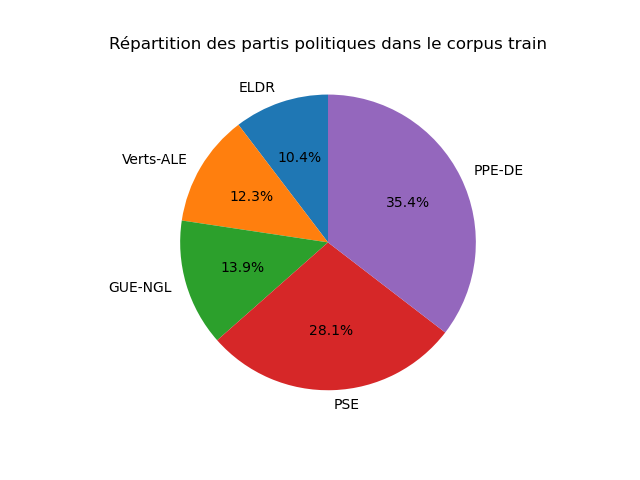
\includegraphics[width=\columnwidth]{../stats/occurences_par_partis_train_camember.png}
    \caption{Répartition des interventions par parti dans la partition train sans doublons}
    \label{fig:camember_dataset}
\end{figure}
\subsection{Prétraitements}
Le texte des interventions a été soumis à un prétraitement simple :\\
\indent(1) Suppresion de la ponctuation\\
\indent(2) Unification de la casse en minuscules\\
\indent(3) Tokenisation\footnote {Une lemmatisation avec la bibliothèque SpaCy a été envisagée,
mais ce corpus multilingue aurait nécessité le chargement de 3 modèles linguistiques
différents et ralongé d'autant le temps de traitement}
\\
Pour résoudre le problème de déséquilibre des classes, nous avons opté pour le \textit{downsampling} afin d'obtenir des classes relativement équilibrées,
en utilisant la fonction \textit{resample} de la bibliothèque Sckit-learn.

\begin{table}[ht]
    \centering
\begin{tabular}{|l|l|l|}
\hline
Parti & Test & train 3 \\ \hline
Moyenne & 3871.4 & 1021.2 \\ \hline
STD & 2149.1 & 569.7 \\ \hline
Min & 2005.0 & 525.0 \\ \hline
1er quartile & 2376.0 & 615.0 \\ \hline
Médiane & 2687.0 & 715.0\\ \hline
3eme quartile & 5431.0 & 1448.0\\ \hline
Max & 6858.0 & 1803.0\\ \hline
\end{tabular}
\caption{Nombres d'intervention par parti par partition}
\label{tab:stats_dataset}
\end{table}


\subsection{Les différents embeddings}

\section{Résultats}

Comme mentionné en introduction, nous avons testé trois méthodes de vectorisation : TF-IDF, doc2vec et BERT
Nous avons utilisé ces vecteurs pour entraîner et comparer 4 modèles différents : Régression logistique, SVM, Random Forest et Perceptron.

\subsection{Vecteurs TF-IDF}

\begin{figure}[t]
  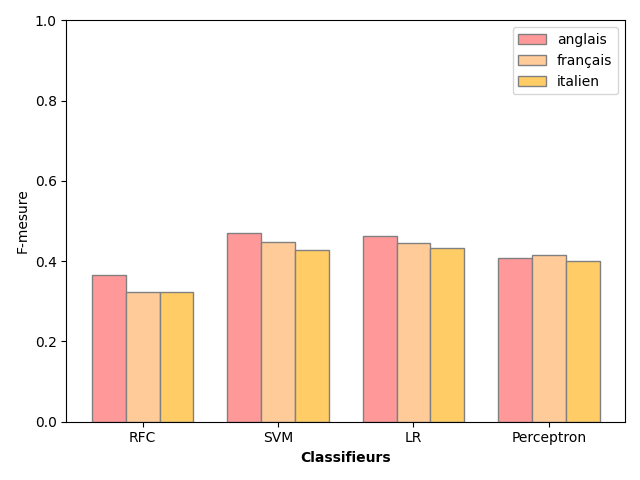
\includegraphics[width=\columnwidth]{assets/comparaison_metriques_tfidf.png}
  \caption{A figure with a caption that runs for more than one line.
    Example image is usually available through the \texttt{mwe} package
    without even mentioning it in the preamble.}
  \label{fig:tfidf_comparison}
\end{figure}

Les meilleurs résultats que nous ayons obtenus sont ceux avec un vectorisation tf-idf.
On peut voir sur la figure~\ref{fig:tfidf_comparison} que nous avons obtenu au mieux : 0.46 en anglais avec un SVM, 0.43 en italien avec une régression linéaire et 0.44 en français avec un SVM.

\section{Discussion et Conclusion}

Les résultats montrent que, sur ce corpus, les vecteurs qui donnent les meilleurs classifieurs sont finalement les moins complexes et les moins denses, c'est-à-dire, les vecteurs \texttt{TF-IDF}. Cela peut s'expliquer de plusieurs façons. Une première raison peut être la nature même des données étudiées : les données de discours du parlement européens sont spécialisée, et contiennent nécessairement des mots relatifs au domaine. Or, \texttt{BERT} est entrainé sur un corpus général. On pourrait envisager de le fine-tuner afin d'obtenir de meilleurs résultats.  \footnote{Il existe également un modèle spécialisé sur le domaine légal, nommé \texttt{LEGAL-BERT}, mais il n'est entraîné que sur l'anglais. Cela pourrait toutefois constituer une recherche ultérieure.} En revanche, le vectoriseur \texttt{TF-IDF} s'adapte au vocabulaire juridique spécifique à ce type de document. Par ailleurs, on peut supposer que la taille relativement réduite des documents peut être à l'origine de la mauvaise qualité des vecteurs obtenus, non seulement avec \texttt{BERT} mais aussi avec \texttt{Doc2Vec}. De plus, les classifieurs que nous lançons sur nos données sont des classifieurs simples, linéaires ou sous forme arbres de décision. Or, les vecteurs complexes générés par réseaux de neurones pourraient nécessiter un réseau de neurones pour la classification ensuite; cela pourrait constituer une perspective pour poursuivre notre expérience. Nous pourrions également imaginer des approches hybrides, qui combineraient les features \texttt{TF-IDF} avec des embeddings \texttt{BERT} pour capturer autant d'informations que nécessaires. De plus, afin d'améliorer les résultats, nous avons envisagé de lancer une \texttt{Grid Seach} pour tuner les hyperparamètres de chacun des classifieurs, mais après quelques tests, le coût computationnel n'a pas su être compensé par une amélioration suffisante de la f-mesure.\footnote{Nous l'avons laissée dans le code malgré tout et il est toujours possible de la faire tourner sur l'ensemble des classifieurs \textit{(cf. \texttt{README.md})}.} Enfin, on remarque que les résultats sont relativement homogènes entre les 3 langues, avec des performances légèrement meilleures pour l'anglais et légèrement en-dessous pour l'italien. 


\section{Bibliographie}

\hypertarget{ref1}{Joseph, Prashob and Yerima, Suleiman Y. 2022. \href{https://www.researchgate.net/profile/Suleiman-Yerima/publication/366445312_A_Comparative_Study_of_Word_Embedding_Techniques_for_SMS_Spam_Detection/links/63a2031641663a23c0714311/A-Comparative-Study-of-Word-Embedding-Techniques-for-SMS-Spam-Detection.pdf}{A comparative study of word embedding techniques for SMS spam detection.} 
In \textit{Proceedings of the 14th International Conference on Computational Intelligence and Communication Networks (CICN)}. Al-Khobar, Saudi Arabia, pages 149-155.}\\



\end{document}
